\documentclass{article}  % Options: 10pt, 11pt, 12pt


\usepackage{amsmath} 
\usepackage{hyperref}
\usepackage[utf8]{inputenc}
\usepackage{graphicx}
\usepackage{array}
\usepackage{indentfirst}
\usepackage{booktabs}
\usepackage[table]{xcolor}  % carrega \rowcolor e \rowcolors
\usepackage{tikz}
\usepackage{caption}
\usepackage{listings}
\usepackage{xcolor} % for color customization
\usepackage[utf8]{inputenc}
\usepackage{float}

\lstdefinelanguage{ReduxAsm}{
  keywords={brzr, ji, ld, st, addi, inc, loadv, addv, not, and, or, xor, add, sub, slr, srr},
  morecomment=[l]{;},
  sensitive=true
}

\lstset{
  language=ReduxAsm,
  basicstyle=\ttfamily\small,
  keywordstyle=\color{blue}\bfseries,
  commentstyle=\color{gray},
  frame=single,
  columns=fullflexible
}

\usetikzlibrary{matrix}

\DeclareMathAlphabet{\mathcal}{OMS}{cmsy}{m}{n}
\SetMathAlphabet{\mathcal}{bold}{OMS}{cmsy}{b}{n}
\title{Trabalho 2 - Arquitetura Redux-V}
\author{EDUARDO KALUF GRR20241770}
\date{\today} 


\begin{document}
    \maketitle
    
    \section{Apresentação}
    
    \setlength{\parindent}{15pt}

    O objetivo deste trabalho é a implementação da \textbf{ISA} \textit{Redux-V}, utilizando as ferramentas \href{https://github.com/gboncoffee/egg}{\textbf{EGG}} e \href{https://github.com/logisim-evolution/logisim-evolution}{\textbf{Logisim}}, visando executar o programa Assembly desenvolvido no "Trabalho 1", além da criação de três instruções adicionais próprias, visando otimizar o problema apresentado.
    Esta \textbf{ISA} é baseada na arquitetura \textit{Risc-V}, porém refatorada a fim de ser mais compacta e amigável para quem está iniciando no mundo da arquitetura de computadores.
    
    Dessa forma, o tamanho da palavra é de oito bits, com endereçamento byte a byte, arquitetura \textbf{Load-Store} e quatro registradores disponíveis.
    Dos oito bits, quatro são utilizados para o \textbf{OPCODE}, permitindo um total de dezesseis instruções para serem exploradas, as quais serão discutidas mais adiante. Além disso, por padrão, existem dois formatos de instrução:

    \begin{table}[h]
      \captionsetup{labelformat=empty, skip=0pt}
      \caption{\textbf{Formato Padrão 1:} Tipo I}
      \centering
      \rowcolors{1}{white}{green!20} 
      \begin{tabular}{|c|*{8}{c|}}
        \hline
        \rowcolor{green!50}
        \multicolumn{9}{|c|}{\textbf{Tipo I}} \\ \hline
        \textbf{Bits} & 7 & 6 & 5 & 4 & 3 & 2 & 1 & 0 \\ \hline
        & \multicolumn{4}{c|}{\textbf{Opcode}} & \multicolumn{4}{c|}{\textbf{Imm.}} \\ \hline
      \end{tabular}
    \end{table}

    \begin{table}[h]
      \captionsetup{labelformat=empty, skip=0pt}
      \caption{\textbf{Formato Padrão 2:} Tipo R}
      \centering
      \rowcolors{1}{white}{blue!20} 
      \begin{tabular}{|c|*{8}{c|}}
        \hline
        \rowcolor{blue!50}
        \multicolumn{9}{|c|}{\textbf{Tipo R}} \\ \hline
        \textbf{Bits} & 7 & 6 & 5 & 4 & 3 & 2 & 1 & 0 \\ \hline
        & \multicolumn{4}{c|}{\textbf{Opcode}} & \multicolumn{2}{c|}{\textbf{Ra}} & \multicolumn{2}{c|}{\textbf{Rb}} \\ \hline
      \end{tabular}
    \end{table}

    \clearpage
    \section{Motivação e Arquitetura}

    A proposta do "Trabalho 1" consistia em criar um programa em \textit{Redux-V} que preenchesse um vetor com números pares (0 a 18) e outro com números ímpares (1 a 19), para posteriormente somar ambos e armazenar os resultados em um terceiro vetor.
    Durante o desenvolvimento do código Assembly no primeiro trabalho, as limitações da arquitetura trouxeram diversos desafios, especialmente devido ao número reduzido de registradores e ao tamanho limitado dos imediatos.

    Dessa forma, ao implementar o "Trabalho 2", tive como objetivo principal facilitar ao máximo a tarefa do programador, evitando a necessidade de programar loops. Além disso, busquei dar caminhos para que o programa pudesse ser mais eficiente, sucinto e organizado.

    Com base nesses objetivos, elaborei as seguintes instruções.

    \subsection{Increment}

    A primeira instrução que implementei foi a instrução "Increment", visando um propósito amplo e genérico. No entanto, busquei torná-la o mais útil possível para o usuário, não limitando sua função apenas ao incremento de 1 em algum registrador específico, por exemplo.

    Para isso, desenvolvi um novo formato de instrução, estabelecendo também um comportamento especial ao utilizar o registrador \textbf{R0}. Essa decisão foi tomada porque incrementar diretamente o \textbf{R0} não teria muito sentido, visto que a instrução addi já consegue cumprir essa tarefa de maneira até mais eficiente.

    \begin{table}[h]
      \captionsetup{labelformat=empty, skip=0pt}
      \caption{\textbf{Formato Novo 1:} Formato para instrução Increment}
      \centering
      \rowcolors{1}{white}{red!20} 
      \begin{tabular}{|c|*{8}{c|}}
        \hline
        \rowcolor{red!50}
        \multicolumn{9}{|c|}{\textbf{Tipo INC}} \\ \hline
        \textbf{Bits} & 7 & 6 & 5 & 4 & 3 & 2 & 1 & 0 \\ \hline
        & \multicolumn{4}{c|}{\textbf{Opcode}} & \multicolumn{2}{c|}{\textbf{Ra}} & \multicolumn{2}{c|}{\textbf{Imm Unsigned}} \\ \hline
      \end{tabular}
    \end{table}
    
    Esta instrução recebe um registrador e um imediato sem sinal, incrementando o valor contido nesse registrador. No entanto, caso o registrador \textbf{R0} seja informado, o incremento ocorrerá em todos os registradores, incluindo o próprio \textbf{R0}. Dessa forma, aproveita-se o que seria um comando duplicado para aprimorar ainda mais a arquitetura.

    \subsection{Load Vector}

    A instrução "Load Vector" vem para resolver o processo de preenchimento dos vetores e, assim como a "Increment", possui algumas características especiais.
    Para que possa ser utilizada corretamente, é necessário que alguns registradores sejam configurados de antemão com valores específicos, seguindo a lógica abaixo:
    
    \begin{itemize}
      \item R0 $\rightarrow$ Endereço de memória do início do vetor;
      \item R1 $\rightarrow$ Incremento de memória que o vetor receberá a cada execução;
      \item R2 $\rightarrow$ Primeiro valor a ser inserido no vetor;
      \item R3 $\rightarrow$ Incremento que o valor de R2 receberá a cada inserção.
    \end{itemize}

    Ademais, ela recebe o tamanho do vetor como parâmetro e utiliza um novo formato de instrução:

    \begin{table}[h]
      \captionsetup{labelformat=empty, skip=0pt}
      \caption{\textbf{Formato Novo 2:} Formato para instruções Vetoriais}
      \centering
      \rowcolors{1}{white}{purple!20} 
      \begin{tabular}{|c|*{8}{c|}}
        \hline
        \rowcolor{purple!50}
        \multicolumn{9}{|c|}{\textbf{Tipo V}} \\ \hline
        \textbf{Bits} & 7 & 6 & 5 & 4 & 3 & 2 & 1 & 0 \\ \hline
        & \multicolumn{4}{c|}{\textbf{Opcode}} & \multicolumn{4}{c|}{\textbf{V-SIZE (Unsigned)}} \\ \hline
      \end{tabular}
    \end{table}

    Vale ressaltar que o tamanho final do vetor será $V\_SIZE \times R1$, e ao fim da execução, $R0$ estará posicionado em $R0 + (R1 \times V\_SIZE)$.

    Exemplo de funcionamento:

    \begin{itemize}
      \item R0 = 27
      \item R1 = 1
      \item R2 = 5
      \item R3 = 10
    \end{itemize}

    \textbf{loadv 4}

    \[
    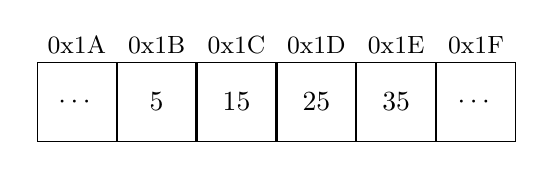
\begin{tikzpicture}
      \matrix[matrix of nodes, 
              nodes in empty cells,
              nodes={draw, minimum size=1cm, anchor=center},
              column sep=0pt] (m) {
        {$\cdots$} & {$5$} & {$15$} & {$25$} & {$35$} & {$\cdots$} \\
      };

      \node[yshift=6pt] at (m-1-1.north) {\small 0x1A};
      \node[yshift=6pt] at (m-1-2.north) {\small 0x1B};
      \node[yshift=6pt] at (m-1-3.north) {\small 0x1C};
      \node[yshift=6pt] at (m-1-4.north) {\small 0x1D};
      \node[yshift=6pt] at (m-1-5.north) {\small 0x1E};
      \node[yshift=6pt] at (m-1-6.north) {\small 0x1F};
    \end{tikzpicture}
    \]

    \subsection{Add Vector}

    Juntamente com a instrução vetorial "Load Vector", criei também a instrução "Add Vector", responsável por somar dois vetores e armazenar o resultado dessa soma em um terceiro.
    Essa instrução utiliza o mesmo formato da "Load Vector", porém os registradores têm funções diferentes, conforme descrito a seguir:

    \begin{itemize}
      \item R0 $\rightarrow$ Endereço de memória do início do primeiro vetor a ser somado;
      \item R1 $\rightarrow$ Endereço de memória do início do segundo vetor a ser somado;
      \item R2 $\rightarrow$ Endereço de memória do início do vetor que armazenará o resultado da soma;
      \item R3 $\rightarrow$ Não possui função nesta operação. Porém, a instrução não garante que o registrador mantenha seu estado inicial;
    \end{itemize}

    Além disso, é necessário que os vetores possuam o mesmo tamanho, pois a soma será feita posição por posição.
    
    Exemplo de funcionamento:


    \begin{itemize}
      \item R0 = 2
      \item R1 = 5
      \item R2 = 8
      \item R3 = 3
    \end{itemize}

    \textbf{addv 3}

    \[
    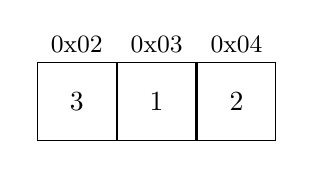
\begin{tikzpicture}
      \matrix[matrix of nodes, 
              nodes in empty cells,
              nodes={draw, minimum size=1cm, anchor=center},
              column sep=0pt] (m) {
        {$3$} & {$1$} & {$2$} \\
      };

      \node[yshift=6pt] at (m-1-1.north) {\small 0x02};
      \node[yshift=6pt] at (m-1-2.north) {\small 0x03};
      \node[yshift=6pt] at (m-1-3.north) {\small 0x04};
    \end{tikzpicture}
    \]

    \[
      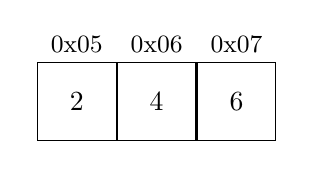
\begin{tikzpicture}
        \matrix[matrix of nodes, 
                nodes in empty cells,
                nodes={draw, minimum size=1cm, anchor=center},
                column sep=0pt] (m) {
          {$2$} & {$4$} & {$6$} \\
        };
  
        \node[yshift=6pt] at (m-1-1.north) {\small 0x05};
        \node[yshift=6pt] at (m-1-2.north) {\small 0x06};
        \node[yshift=6pt] at (m-1-3.north) {\small 0x07};
      \end{tikzpicture}
    \]

    \[
      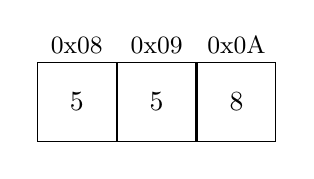
\begin{tikzpicture}
        \matrix[matrix of nodes, 
                nodes in empty cells,
                nodes={draw, minimum size=1cm, anchor=center},
                column sep=0pt] (m) {
          {$5$} & {$5$} & {$8$} \\
        };
  
        \node[yshift=6pt] at (m-1-1.north) {\small 0x08};
        \node[yshift=6pt] at (m-1-2.north) {\small 0x09};
        \node[yshift=6pt] at (m-1-3.north) {\small 0x0A};
      \end{tikzpicture}
    \]
  
    \subsection{Resultado}

    Desta forma, após a implementação dessas três novas instruções ficamos com a seguinte ISA:

    \begin{table}[H]
      \rowcolors{1}{white}{gray!20} 
      \noindent\hspace*{-1.75cm}%
      \begin{tabular}{|c|*{4}{c|}}
        \hline
        \rowcolor{gray!50}
        \multicolumn{1}{|c|}{\textbf{Opcode}} & \multicolumn{1}{|c|}{\textbf{Tipo}} & \multicolumn{1}{|c|}{\textbf{Mnemonic}} & \multicolumn{1}{|c|}{\textbf{Nome}}                   & \multicolumn{1}{|c|}{\textbf{Operação}}  \\ \hline
        \multicolumn{1}{|c|}{\textbf{0000}}    & \multicolumn{1}{c|}{\textbf{R}}     & \multicolumn{1}{c|}{\textbf{brzr}}      & \multicolumn{1}{c|}{\textbf{Branch On Zero Register}} & \multicolumn{1}{c|}{\textbf{if (R[ra] == 0) PC = R[rb]}}  \\ \hline
        \multicolumn{1}{|c|}{\textbf{0001}}    & \multicolumn{1}{c|}{\textbf{I}}     & \multicolumn{1}{c|}{\textbf{ji}}        & \multicolumn{1}{c|}{\textbf{Jump Immediate}}          & \multicolumn{1}{c|}{\textbf{PC = PC + Imm.}}  \\ \hline
        \multicolumn{1}{|c|}{\textbf{0010}}    & \multicolumn{1}{c|}{\textbf{R}}     & \multicolumn{1}{c|}{\textbf{ld}}        & \multicolumn{1}{c|}{\textbf{Load}}                    & \multicolumn{1}{c|}{\textbf{R[ra] = M[ R[rb] ]}}  \\ \hline
        \multicolumn{1}{|c|}{\textbf{0011}}    & \multicolumn{1}{c|}{\textbf{R}}     & \multicolumn{1}{c|}{\textbf{st}}        & \multicolumn{1}{c|}{\textbf{Store}}                   & \multicolumn{1}{c|}{\textbf{M[ R[rb] ] = R[ra]}}  \\ \hline
        \multicolumn{1}{|c|}{\textbf{0100}}    & \multicolumn{1}{c|}{\textbf{I}}     & \multicolumn{1}{c|}{\textbf{addi}}      & \multicolumn{1}{c|}{\textbf{Add Immediate}}           & \multicolumn{1}{c|}{\textbf{R[0] = R[0] + Imm.}}  \\ \hline
        \multicolumn{1}{|c|}{\textbf{0101}}    & \multicolumn{1}{c|}{\textbf{V}}     & \multicolumn{1}{c|}{\textbf{loadv}}     & \multicolumn{1}{c|}{\textbf{Load Vector}}             & \multicolumn{1}{c|}{\textbf{Micro-Code-1}}  \\ \hline
        \multicolumn{1}{|c|}{\textbf{0110}}    & \multicolumn{1}{c|}{\textbf{V}}     & \multicolumn{1}{c|}{\textbf{addv}}      & \multicolumn{1}{c|}{\textbf{Add Vector}}              & \multicolumn{1}{c|}{\textbf{Micro-Code-2}}  \\ \hline
        \multicolumn{1}{|c|}{\textbf{0111}}    & \multicolumn{1}{c|}{\textbf{INC}}   & \multicolumn{1}{c|}{\textbf{inc}}       & \multicolumn{1}{c|}{\textbf{Increment}}               & \multicolumn{1}{c|}{\textbf{Ra = Ra + Imm Unsigned}}  \\ \hline
        \multicolumn{1}{|c|}{\textbf{1000}}    & \multicolumn{1}{c|}{\textbf{R}}     & \multicolumn{1}{c|}{\textbf{not}}       & \multicolumn{1}{c|}{\textbf{Not}}                     & \multicolumn{1}{c|}{\textbf{R[ra] = not R[rb]}}  \\ \hline
        \multicolumn{1}{|c|}{\textbf{1001}}    & \multicolumn{1}{c|}{\textbf{R}}     & \multicolumn{1}{c|}{\textbf{and}}       & \multicolumn{1}{c|}{\textbf{And}}                     & \multicolumn{1}{c|}{\textbf{R[ra] = R[ra] and R[rb]}}  \\ \hline
        \multicolumn{1}{|c|}{\textbf{1010}}    & \multicolumn{1}{c|}{\textbf{R}}     & \multicolumn{1}{c|}{\textbf{or}}        & \multicolumn{1}{c|}{\textbf{Or}}                      & \multicolumn{1}{c|}{\textbf{R[ra] = R[ra] or R[rb]}}  \\ \hline
        \multicolumn{1}{|c|}{\textbf{1011}}    & \multicolumn{1}{c|}{\textbf{R}}     & \multicolumn{1}{c|}{\textbf{xor}}       & \multicolumn{1}{c|}{\textbf{Xor}}                     & \multicolumn{1}{c|}{\textbf{R[ra] = R[ra] xor R[rb]}}  \\ \hline
        \multicolumn{1}{|c|}{\textbf{1100}}    & \multicolumn{1}{c|}{\textbf{R}}     & \multicolumn{1}{c|}{\textbf{add}}       & \multicolumn{1}{c|}{\textbf{Add}}                     & \multicolumn{1}{c|}{\textbf{R[ra] = R[ra] + R[rb]}}  \\ \hline
        \multicolumn{1}{|c|}{\textbf{1101}}    & \multicolumn{1}{c|}{\textbf{R}}     & \multicolumn{1}{c|}{\textbf{sub}}       & \multicolumn{1}{c|}{\textbf{Sub}}                     & \multicolumn{1}{c|}{\textbf{R[ra] = R[ra] - R[rb]}}  \\ \hline
        \multicolumn{1}{|c|}{\textbf{1110}}    & \multicolumn{1}{c|}{\textbf{R}}     & \multicolumn{1}{c|}{\textbf{slr}}       & \multicolumn{1}{c|}{\textbf{Shift Left Register}}     & \multicolumn{1}{c|}{\textbf{R[ra] = R[ra] << R[rb]}}  \\ \hline
        \multicolumn{1}{|c|}{\textbf{1111}}    & \multicolumn{1}{c|}{\textbf{R}}     & \multicolumn{1}{c|}{\textbf{srr}}       & \multicolumn{1}{c|}{\textbf{Shift Right Register }}   & \multicolumn{1}{c|}{\textbf{R[ra] = R[ra] >> R[rb]}}  \\ \hline
      \end{tabular}
    \end{table}

    Os microcódigos executados pelas funções são

    \renewcommand{\lstlistingname}{Microcódigo}
    \begin{lstlisting}[caption={Load Vector}]
    \begin{lstlisting}
      _loop:
        st r2, r0
        add r0, r1
        add r2, r3
        ji _loop
    \end{lstlisting}
      
    \renewcommand{\lstlistingname}{Microcódigo}
    \begin{lstlisting}[caption={Add Vector}]
    \begin{lstlisting}
      _program2:
        ld r0, r0   ;; (r0, rx)
        ld r1, r1   ;; (r0, ry)
        add r3, r0  ;; (rx + ry -> r3)
        st r3, r2
        inc 1, r0   ;; (r0, r1, r2, r3 += 1)
        ji _program2
    \end{lstlisting}

    \clearpage
    \section{Assembly}

    Após as modificações feitas, a solução para o problema dos vetores se tornou muito mais sucinta, fácil de entender e otimizada.

    \captionsetup[lstlisting]{labelformat=empty}
    \renewcommand{\lstlistingname}{}
    \begin{lstlisting}[caption={Código do "Trabalho 1"}]
    _setupMemoria:
      ;; Mem[-1] = (COMECO DO VETOR A) (0x70) (112)
      addi 0
      addi 7
      add r2, r0
      addi -3
      slr r2, r0
      addi -5
      st r2, r0
      ;;

      ;; Mem[-3] = COUNTER (0x0a)
      addi 6
      addi 5
      add r1, r0
      sub r0, r0
      addi -3
      st r1, r0
      ;;

      ;; Mem[-4] = 10 FIXO (0x0a)
      addi -1
      st r1, r0
      ;;

      ;; Mem[-5] = 20 FIXO (0x14)
      addi -1
      add r1, r1
      st r1, r0
      ;;

      ;; Mem[-2] = ENTRADA DO "loopSoma" 
      ;; (INICIO DO VETOR (r2) N DE INSTRUCOES DO "loopSoma") (0x52)
      sub r0, r0
      addi -2
      add r3, r0
      sub r2, r1
      addi 7
      addi 5
      sub r2, r0
      st r2, r3
      ;;

    _setupLoopEven:

      ;; r1 = 1 (0x01)
      sub r0, r0
      sub r1, r1
      addi 1
      add r1, r0
      ;;

      ;; r3 = (FINAL DO VETOR A) (0x79) (121)
      addi -2
      ld r0, r0
      addi 7
      addi 2
      sub r3, r3
      add r3, r0
      ;;

      ;; r2 = SAIDA DO LOOP EVEN (0x34)
      sub r0, r0
      sub r2, r2
      addi 6
      add r2, r0
      addi -3
      slr r2, r0
      addi 1
      add r2, r0
      sub r0, r0
      ;;

      ;; r0 = 20 (0x14)
      addi -5
      ld r0, r0
      ;;

    _loopEven:
      addi -2     ;; r0 -= 2
      st r0, r3   ;; A[r3] = r0 
      sub r3, r1  ;; r3 -= 1
      brzr r0, r2 ;; if (r0 == 0) break
      ji _loopEven

    _setupLoopOdd:

      ;; r2 = SAIDA DO LOOP ODD (0x43)
      sub r2, r2
      addi 4
      slr r0, r0
      addi 3
      add r2, r0
      ;;

      ;; r3 = (FINAL DO VETOR B) (0x83) (131)
      sub r0, r0
      addi -5
      ld r0, r0
      add r3, r0
      ;;

      ;; r1 JA E IGUAL A 1  (0x01)

      ;; r0 JA E IGUAL A 20 (0x14)

    _loopOdd:
      addi -1     ;; r0 -= 1
      st r0, r3   ;; B[r3] = r0
      sub r3, r1  ;; r3 -= 1
      addi -1     ;; r0 -= 1
      brzr r0, r2 ;; if (r0 == 0) break
      ji _loopOdd

    _setupLoopZero:

      ;; r3 = (FINAL DO VETOR R) (0x8D) (141)
      ;; r1 = COUNTER (0x0A)
      addi -3
      ld r1, r0
      addi -2
      ld r0, r0
      add r3, r0
      ;;

      ;; r2 = SAIDA DO LOOP ZERO (POSICAO -2 da memoria) (0x52)
      sub r0, r0
      addi -2
      ld r2, r0
      ;;

    _loopZero:
      sub r0, r0  ;; r0 = 0
      st r0, r3   ;; R[r3] = r0
      addi 1      ;; r0 = 1
      sub r3, r0  ;; r3 -= 1
      sub r1, r0  ;; r1 -= 1
      brzr r1, r2 ;; if (r1 == 0) break
      ji _loopZero

    _loopSum:
      sub r0, r0  ;; r0 = 0
      addi -1     ;; r0 = -1
      ld r3, r0   ;; r3 = Mem[-1] (COMECO DO VETOR A)
      addi 2      ;; r0 = 1
      add r3, r0  ;; r3 += 1
      addi -2     ;; r0 = -1
      st r3, r0   ;; Mem[-1] = (POSICAO ATUAL DO VETOR A + 1)
      addi 2      ;; r0 = 1
      sub r3, r0  ;; r3 -= 1 (POSICAO ATUAL DO VETOR A) 
      addi -5     ;; r0 = -4
      ld r0, r0   ;; r0 = Mem[-4] (0x0a)
      ld r1, r3   ;; r1 = A[r3]
      add r3, r0  ;; r3 += 10
      ld r2, r3   ;; r2 = B[r3]
      add r1, r2  ;; r1 = A[r3] + B[r3]
      add r3, r0  ;; r3 += 10
      st r1, r3   ;; R[r3] = A[r3] + B[r3]
      sub r0, r0  ;; r0 = 0
      addi -3     ;; r0 = -3
      ld r1, r0   ;; r1 = Mem[-3] (COUNTER)
      addi 4      ;; r0 = 1
      sub r1, r0  ;; r1 -= 1
      addi -4     ;; r0 = -3
      st r1, r0   ;; Mem[-3] = COUNTER - 1
      not r1, r1  ;; r1 = !r1 (zero a nao ser na interacao de saida)
      addi 1      ;; r0 = -2
      ld r2, r0   ;; r2 = Mem[-2] ENTRADA DO "loopSoma"
      brzr r1, r2 ;; if (r1 == 0) continue

    _loopInfinite:
      addi 0 
      ji _loopInfinite

    \end{lstlisting}

    \clearpage
    \captionsetup[lstlisting]{labelformat=empty}
    \renewcommand{\lstlistingname}{}
    \begin{lstlisting}[caption={Código do "Trabalho 2", Otimizado com as novas instruções}]
    inc r1, 1
    inc r3, 2
    addi 4
    slr r0, r0
    loadv 10
    sub r2, r2
    inc r2, 1
    loadv 10
    sub r2, r2
    add r2, r0
    addi -7
    addi -3
    sub r1, r1
    add r1, r0
    addi -7
    addi -3
    addv 10
    _loopInfinite:
        addi 0 
        ji _loopInfinite
    \end{lstlisting}

    \clearpage
    \section{Implementação e Organização}

    Essa seção será dividida entre a implementação padrão do \textit{Redux-V}, a implementação da \textbf{ULA} e a implementação das três funções adicionais. Ao final, serão apresentadas a tabela de controle e informações adicionais.

    \subsection{Monociclo}

    O monociclo é simples e compacto, sendo implementado com o uso de uma \textbf{RAM} de duas portas e uma memória de controle, composta pelos seguintes módulos:

    \begin{itemize}
      \item Program Counter
      \item Dual-Port RAM
      \item Memória de Controle
      \item Banco de Registradores
      \item ULA
    \end{itemize}

    A seguir, apresenta-se o datapath desta arquitetura em um diagrama de blocos simplificado.

    \vspace{1cm}
    \noindent\hspace*{-4cm}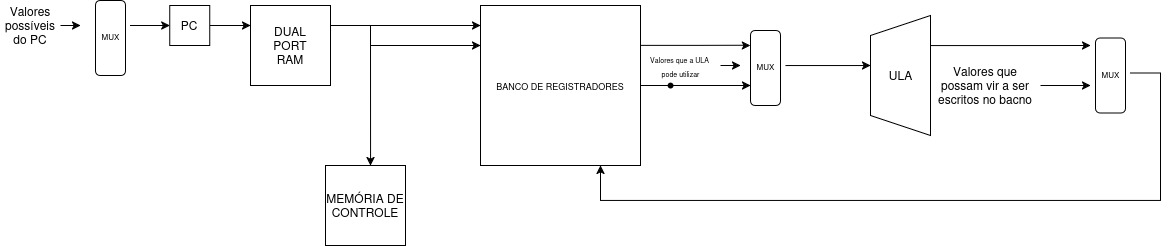
\includegraphics[scale=0.5]{datapath.jpg}
    \vspace{1cm}

    A \textbf{ULA} foi projetada para conter oito operações, além de uma saída \textbf{ZERO}, que detecta se o \textbf{RA} é nulo, utilizada em casos de branching

    A seguir, apresenta-se o projeto da ULA em um diagrama de blocos simplificado.
    
    \vspace{1cm}
    \noindent\hspace*{2cm}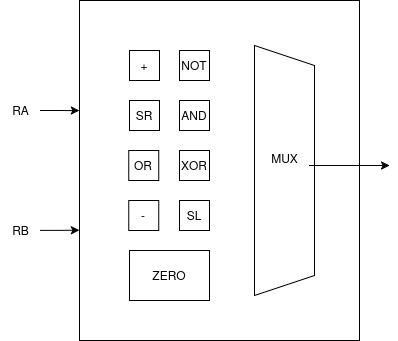
\includegraphics[scale=0.5]{ULA.jpg}
    \vspace{3cm}

    Os códigos de controle da ULA:

    \begin{table}[H]
      \rowcolors{1}{white}{gray!20} 
      \noindent\hspace*{3cm}%
      \begin{tabular}{{|c c|}}
        \hline
        \rowcolor{gray!50}
        \multicolumn{1}{|c}{\textbf{Operação}}           & \multicolumn{1}{c|}{\textbf{OP\_ULA}} \\ \hline
        \multicolumn{1}{|c}{\textbf{Not}}                & \multicolumn{1}{c|}{\textbf{000}} \\ \hline
        \multicolumn{1}{|c}{\textbf{And}}                & \multicolumn{1}{c|}{\textbf{001}} \\ \hline
        \multicolumn{1}{|c}{\textbf{Or}}                 & \multicolumn{1}{c|}{\textbf{010}} \\ \hline
        \multicolumn{1}{|c}{\textbf{Xor}}                & \multicolumn{1}{c|}{\textbf{011}} \\ \hline
        \multicolumn{1}{|c}{\textbf{Soma}}               & \multicolumn{1}{c|}{\textbf{100}} \\ \hline
        \multicolumn{1}{|c}{\textbf{Subtração}}          & \multicolumn{1}{c|}{\textbf{101}} \\ \hline
        \multicolumn{1}{|c}{\textbf{Shift left lógico}}  & \multicolumn{1}{c|}{\textbf{110}} \\ \hline
        \multicolumn{1}{|c}{\textbf{Shift right lógico}} & \multicolumn{1}{c|}{\textbf{111}} \\ \hline
      \end{tabular}
    \end{table}

    \subsection{Extensão}

    Para implementar as três instruções adicionais, além dos novos sinais de controle introduzidos no monociclo tradicional, uma nova área foi adicionada para atender às necessidades específicas dessas instruções. Essa nova área contém:

    \begin{itemize}
      \item Um novo Program Counter
      \item Uma nova memória de instruções
      \item Dois contadores
    \end{itemize}

    \subsubsection{Increment}

    A instrução "Increment" opera de forma linear para os registradores \textbf{R1} a \textbf{R3}. Ela recebe um valor imediato fornecido pelo campo que normalmente indicaria o endereço do registrador \textbf{RB}, realiza a soma desse imediato com o valor do registrador \textbf{RA} na \textbf{ULA}, e então armazena o resultado de volta no próprio registrador \textbf{RA}.

    Caso o registrador passado seja \textbf{R0}, o sinal de controle "INC\_ALL" é ativado, habilitando a escrita em todos os registradores. Dessa forma, somadores internos ao próprio banco de registradores realizam o incremento diretamente em cada um deles.

    \subsubsection{Load Vector}

    A instrução "Load Vector" ativa o sinal de controle "LOAD\_V", que altera o fluxo de operação do processador. Com isso, as instruções passam a ser buscadas a partir da memória secundária. Além disso, um contador é inicializado com o tamanho do vetor que será carregado.

    A partir disso, um Microcódigo que preenche o vetor começa a operar. Esse Microcódigo consiste em um loop simples, que finaliza com a execução de uma instrução do tipo \textbf{JI}. A cada iteração, com a execução do \textbf{JI}, o contador é reduzido em uma unidade. Quando o contador chega a zero, o processador retorna ao fluxo normal de execução.

    \subsubsection{Add Vector}

    De forma similar, a instrução "Add Vector" também modifica o fluxo do processador, ativando um contador e executando um outro Microcódigo. Contudo, há diferenças na forma como as instruções "Load" e "Add" operam dentro desse Microcódigo.
    
    No caso da instrução "Load", o registrador \textbf{RB} passa a ser interpretado de outra forma: o \textbf{R0} passa a ser \textbf{Rx} e o \textbf{R1} passa a ser \textbf{Ry}, um par adicional de registradores utilizados exclusivamente durante este Microcódigo.
    
    Já a instrução "Add", a operação ocorre sempre somando os valores dos registradores \textbf{Rx}, \textbf{Ry} e armazenando o resultado no registrador \textbf{R3}.
    
    \noindent\hspace*{0cm}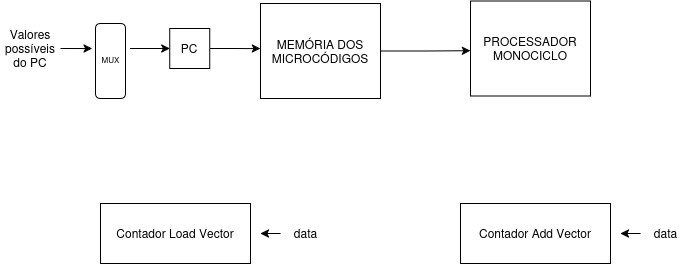
\includegraphics[scale=0.5]{extensao.jpg}
    \vspace{1cm}   

    \subsection{Controle}

    Finalmente então, temos os controles tabelados:

    \begin{table}[H]
      \captionsetup{labelformat=empty, skip=0pt}
      \caption{\textbf{Bits de Controle}}
      \centering
      \noindent\hspace*{-3cm}
      \resizebox{1.5\textwidth}{!}{
        \begin{tabular}{@{} l c c c c c c c c c c c c c @{}}
          \toprule
          Mnemonic & OPCODE & ADDV & INC & LOADV & LOAD & BRZR & JI & ADDI & W\_MEM & IMM\_ULA & OP\_ULA & W\_RG & HEX\_VALUE \\
          \midrule
          brzr   & 0000 & 0 & 0 & 0 & 0 & 1 & 0 & 0 & 0 & 0 & 000 & 0 & 0x100 \\
          ji     & 0001 & 0 & 0 & 0 & 0 & 0 & 1 & 0 & 0 & 1 & 100 & 0 & 0x098 \\
          ld     & 0010 & 0 & 0 & 0 & 1 & 0 & 0 & 0 & 0 & 0 & 000 & 1 & 0x201 \\
          st     & 0011 & 0 & 0 & 0 & 0 & 0 & 0 & 0 & 1 & 0 & 000 & 0 & 0x020 \\
          addi   & 0100 & 0 & 0 & 0 & 0 & 0 & 0 & 1 & 0 & 1 & 100 & 1 & 0x059 \\
          loadv  & 0101 & 0 & 0 & 1 & 0 & 0 & 0 & 0 & 0 & 0 & 000 & 0 & 0x400 \\
          addv   & 0110 & 1 & 0 & 0 & 0 & 0 & 0 & 0 & 0 & 0 & 000 & 0 & 0x1000 \\
          inc    & 0111 & 0 & 1 & 0 & 0 & 0 & 0 & 0 & 0 & 0 & 100 & 1 & 0x809 \\
          not    & 1000 & 0 & 0 & 0 & 0 & 0 & 0 & 0 & 0 & 0 & 000 & 1 & 0x001 \\
          and    & 1001 & 0 & 0 & 0 & 0 & 0 & 0 & 0 & 0 & 0 & 001 & 1 & 0x003 \\
          or     & 1010 & 0 & 0 & 0 & 0 & 0 & 0 & 0 & 0 & 0 & 010 & 1 & 0x005 \\
          xor    & 1011 & 0 & 0 & 0 & 0 & 0 & 0 & 0 & 0 & 0 & 011 & 1 & 0x007 \\
          add    & 1100 & 0 & 0 & 0 & 0 & 0 & 0 & 0 & 0 & 0 & 100 & 1 & 0x009 \\
          sub    & 1101 & 0 & 0 & 0 & 0 & 0 & 0 & 0 & 0 & 0 & 101 & 1 & 0x00B \\
          slr    & 1110 & 0 & 0 & 0 & 0 & 0 & 0 & 0 & 0 & 0 & 110 & 1 & 0x00D \\
          srr    & 1111 & 0 & 0 & 0 & 0 & 0 & 0 & 0 & 0 & 0 & 111 & 1 & 0x00F \\
          \bottomrule
        \end{tabular}
      }
    \end{table}

    \clearpage
    \section{EGG e Redux-K}

    Juntamente com a implementação das instruções no \textbf{Logisim}, o emulador \textbf{EGG} também foi modificado para interpretá-las corretamente.
    Dessa forma, dou vida à arquitetura \textit{Redux-K} (\textit{Redux-V} versão Kaluf), que agora pode ser utilizada como qualquer outra arquitetura disponível no emulador.
    \vspace{1cm}

    \href{https://github.com/Eduardo-Kaluf/redux-K}{\textbf{REDUX-K}}

    \section{Conclusão}

    Com o processador finalizado, foi possível perceber novas formas de se trabalhar com o hardware, as limitações de uma \textbf{ISA} reduzida e ao mesmo tempo a ampla gama de possibilidades de melhorias e inovações que ela oferece.

    Trabalhar na implementação do \textit{ReduxV} e enfrentar o desafio da soma de vetores proporcionou diversas experiências técnicas, que me levaram por caminhos diferentes dos que estou acostumado a lidar. Isso ampliou minha visão e sensibilidade em relação ao funcionamento dos processadores e do hardware.
    
    Foi um processo interessante e muito proveitoso. 

\end{document} 